\documentclass[11pt]{scrartcl}
\usepackage[sexy]{{Style_Files/evan}}

\usepackage{{Style_Files/NMC}}
\usepackage[subpreambles=true]{standalone}
\usepackage{import}

\begin{document}
\title{NMC Problem Set \#5}
\date{Sep. 18, 2022} 
\maketitle

\section*{Welcome!}

This is a selection of interesting problems derived from curious thoughts, curated so you can nibble on them throughout the week! The point of this document is to introduce you to fun puzzles that require thinking. We recommend you try the ones that you find interesting! Feel free to work on them with others (even us teachers!). Harder problems are marked with chilies (\fullchili), in case you want to challenge yourself.
\newline\newline
Have fun! \textit{Note: New variants on these problems may be released throughout the week. Remember to check back once in a while!}
    
\section{Algebra}
\begin{enumerate}[label=\textbf{A\arabic*}.]
    \item \textbf{Pigeonhole Principle} \newline
    The Pigeonhole Principle states that if you have $n$ objects and $k$ containers such that $n>k$ and all $n$ objects are placed in said containers, then at least one container has at least $\floor{\frac{n}{k}}$ things in it. Here's an assortment of problems all related to the pigeonhole principle in some shape or form!
    \begin{enumerate}
        \item Suppose that in a party of $n$ people where some people shake hands, show that there are at least two people who have shaken hands with the same number of people!
        
        \item What is the size of the largest subset $\SA$ of $\{1, 2, \dots, 2n\}$ such that for all choices of $a, b \in \SA$, $a$ does not divide $b$?
        
        \item (\halfchili) (Japan 1997) Prove that among any $10$ points in a circle of diameter $5$, there exists at least two points with a distance less than $2$ from each other.
        
        \item (\fullchili) Pick $13$ real numbers. Show that there are two of them, call them $x$ and $y$, such that
        \[ 0 < \frac{x - y}{1 + xy} < 2 - \sqrt{3}. \]
        
        \item (\fullchili\,$\times$\,2) Prove that every positive integer divides into at least one Fibonacci number.
    \end{enumerate}
\end{enumerate}

\newpage
\section{Combinatorics}
\begin{enumerate}[label=\textbf{C\arabic*}.]
    \item \textbf{Robot Shenanigans} \newline
    The OneShot Math Group has created a robot to traverse the barrens! To keep things simple, MPK feeds the robot follows a simple set of instructions, consisting of the moves "up," "down," "left," and "right." Once the robot finishes the list of moves given to it, it will loop the moveset, where the cycle continues until it reaches its destination.
    
    Below is a sample maze!
    \begin{figure}[h]
        \centering
        \includegraphics[width = 4cm]{Diagrams/Week 5 Robot Maze 1.tex}
    \end{figure}
    The robot starts on the green box, and it wants to get to the red box. Here, MPK only has to teach the robot $2$ moves ("right, up") for it to reach its destination! The following puzzles ask for you to determine the least number of moves that MPK has to give the robot to complete the respective mazes.
    
    \begin{enumerate}
        \item \begin{tabular}{C{11cm}}
            \includegraphics[width = 6cm]{Diagrams/Week 5 Robot Maze 2.tex}
        \end{tabular}
        
        \item \begin{tabular}{C{11cm}}
            \includegraphics[width = 3.58cm]{Diagrams/Week 5 Robot Maze 3.tex}
        \end{tabular}
        
        \item Now, consider the above puzzles, but MPK is now able to teach the robot to "turn right" or "turn left." If the robot turns, all of its moves will now be according to the new orientation! What's the least number of moves needed now?
    \end{enumerate}
\end{enumerate}

\newpage
\section{Geometry}
\begin{enumerate}[label=\textbf{G\arabic*}.]
    \item (\fullchili) \textbf{Origami Trisection} \newline
    The \href{https://en.wikipedia.org/wiki/Huzita\%E2\%80\%93Hatori_axioms}{Huzita-Hatori Axioms} are a list of "legal folds" defined for origami construction! Below, we have a diagram illustrating how to trisect a given angle a square sheet of paper. Prove that such a construction actually works, despite the fact that you can't trisect an angle with a compass and straightedge!
    \newline
    \begin{figure}[h]
        \centering
        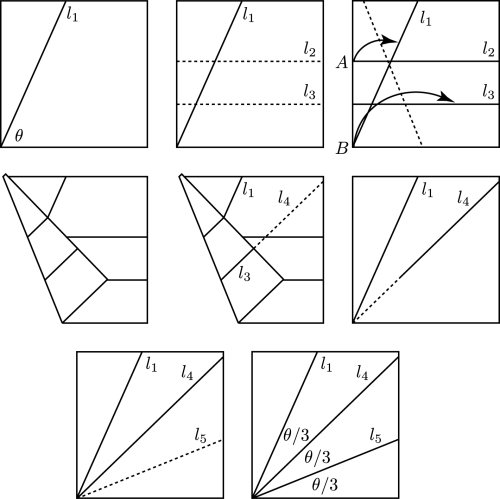
\includegraphics[width = 12cm]{Diagrams/Origami Trisection.png}
        \caption{Source: \href{https://divisbyzero.files.wordpress.com/2012/06/origamitrisection.png?w=500}{Thanks, Dave Richeson!}}
        \label{fig:Origami_Trisection}
    \end{figure}
\end{enumerate}

\newpage
\section{Number Theory}
\begin{enumerate}[label=\textbf{N\arabic*}.]
    \item \textbf{Fermat's Little Theorem} \newline
    Fermat's Little Theorem is usually as
    \[ a^p \equiv a \pmod{p}, \]
    where $a$ is an integer and $p$ is a prime. When $a$ is not a multiple of $p$, this is also equivalent to
    \[ a^{p-1} \equiv 1 \pmod{p}. \]
    Let's prove it using induction!
    \begin{enumerate}
        \item First, prove that
        \[ (x + y)^p \equiv x^p + y^p \pmod{p} \]
        for all primes $p$. Consider writing out the left hand side using binomial expansion!
        
        \item Using the lemma above, prove that Fermat's little theorem holds for all integers $a$. \footnote{Hint: Consider proving the case $a^p \equiv a \pmod{p}$. The other version follows immediately.}
    \end{enumerate}
    
    This concludes the proof!
    
    \begin{enumerate}[start = 3]
        \item (\fullchili) Arky incorrectly remembered Fermat's Little Theorem as
        \[ a^{n+1} \equiv 1 \pmod{n}. \]
        Describe the set of all $n$ for which the above is true!
    \end{enumerate}
    
    \item (\fullchili) \textbf{A Funky Factorial} \newline
    Prove the following identity:
    \[ n! = \prod_{k = 1}^n \lcm \left(1, 2, \dots, \floor{\frac{n}{k}}\right). \]
\end{enumerate}
\end{document}
